\section{Completely Fair Scheduling}

The Completely Fair Scheduler (CFS) was introduced as a solution to address limitations in the original $O(1)$ scheduler, which imposed rigid decisions regarding timeslices and priorities. 
The $O(1)$ scheduler struggled to balance CPU-bound and I/O-bound tasks effectively, leading to issues like excessive context switching, especially for low-priority, compute-heavy processes.
CFS takes a more dynamic approach, adjusting timeslices based on system load and task priority.

The key features are the following: 
\begin{enumerate}
    \item \textit{Dynamic timeslice assignment}: CFS assigns each process a timeslice proportional to the system load, ensuring efficient distribution of CPU resources. 
        This approach minimizes context switching overhead for compute-bound processes while also accommodating I/O-bound processes more effectively.
    \item \textit{Fair CPU time allocation}: each process's timeslice ($\tau_p$) is computed using the formula:
        \[\tau_p=\max\left(\dfrac{\lambda_p\bar{\tau}}{\sum\lambda_i},\mu\right)\]
        Here, $\lambda_p$ is the weight of the process (derived from its priority), $\bar{\tau}$ is the configurable schedule latency (default: 6ms), and $\mu$ is the minimum granularity (default: 0.75ms). 
        This formula ensures that processes receive a fair share of CPU time based on their priority, with the minimum granularity parameter guaranteeing that even low-priority tasks get some CPU time.
    \item \textit{Exponential weighting}: the process weight $\lambda_i$ is calculated using an exponential formula:
        \[\lambda_i=kb^{v_i}\]
        Here, $k = 1024$ and $b = 1.25$, and $v_i$ is the process's nice value (priority).
        This gives finer control over process prioritization and CPU allocation.
    \item \textit{vruntime ($\rho$) for fairness}: CFS tracks a virtual runtime ($\rho$) for each process, which reflects how much CPU time a process has used relative to its weight. 
        Lower $\rho$ values indicate higher priority, and tasks with higher weights typically have lower $\rho$. 
        The goal is to balance $\rho$ values across all processes, ensuring that each task receives its fair share of CPU time, even when priorities differ. 
        The relationship is described by:
        \[\Delta\rho_p=\dfrac{\tau_p}{\lambda_p}=\dfrac{\bar{\tau}}{\sum\lambda_i}\]
        This formula highlights that the increase in a process's $\rho$ over time depends only on the total weight of all runnable processes, allowing for equitable CPU distribution.
\end{enumerate}
The purpose of CFS is to ensure fair CPU time allocation among all processes. 
It achieves this by scaling task priorities using the nice value, which adjusts the proportion of CPU time a process receives based on its priority. 
This design helps balance the needs of different processes, promoting fairness across the system.

However, CFS has some limitations. One major drawback is its latency sensitivity. 
CFS struggles to handle processes that require quick access to the CPU but only need short bursts of processing time. 
It lacks a dedicated mechanism to account for such latency-sensitive tasks. 
Additionally, while real-time scheduling classes can address latency concerns, they are privileged and can disrupt the fairness of the system by monopolizing CPU resources, making them an imperfect solution.
\begin{example}
    The diagram below illustrates a time chart for the Completely Fair Scheduler (CFS) with three tasks, labeled $A$, $B$, and $C$, each running for eight time units. 
    Task $A$ and Task $B$ both have a weight ($\lambda$) of 1, while Task $C$ has a higher weight of 2. 
    At the beginning, none of the tasks have any priority adjustments, indicated by the initial virtual runtime ($\rho$) being 0.
    \begin{figure}[H]
        \centering
        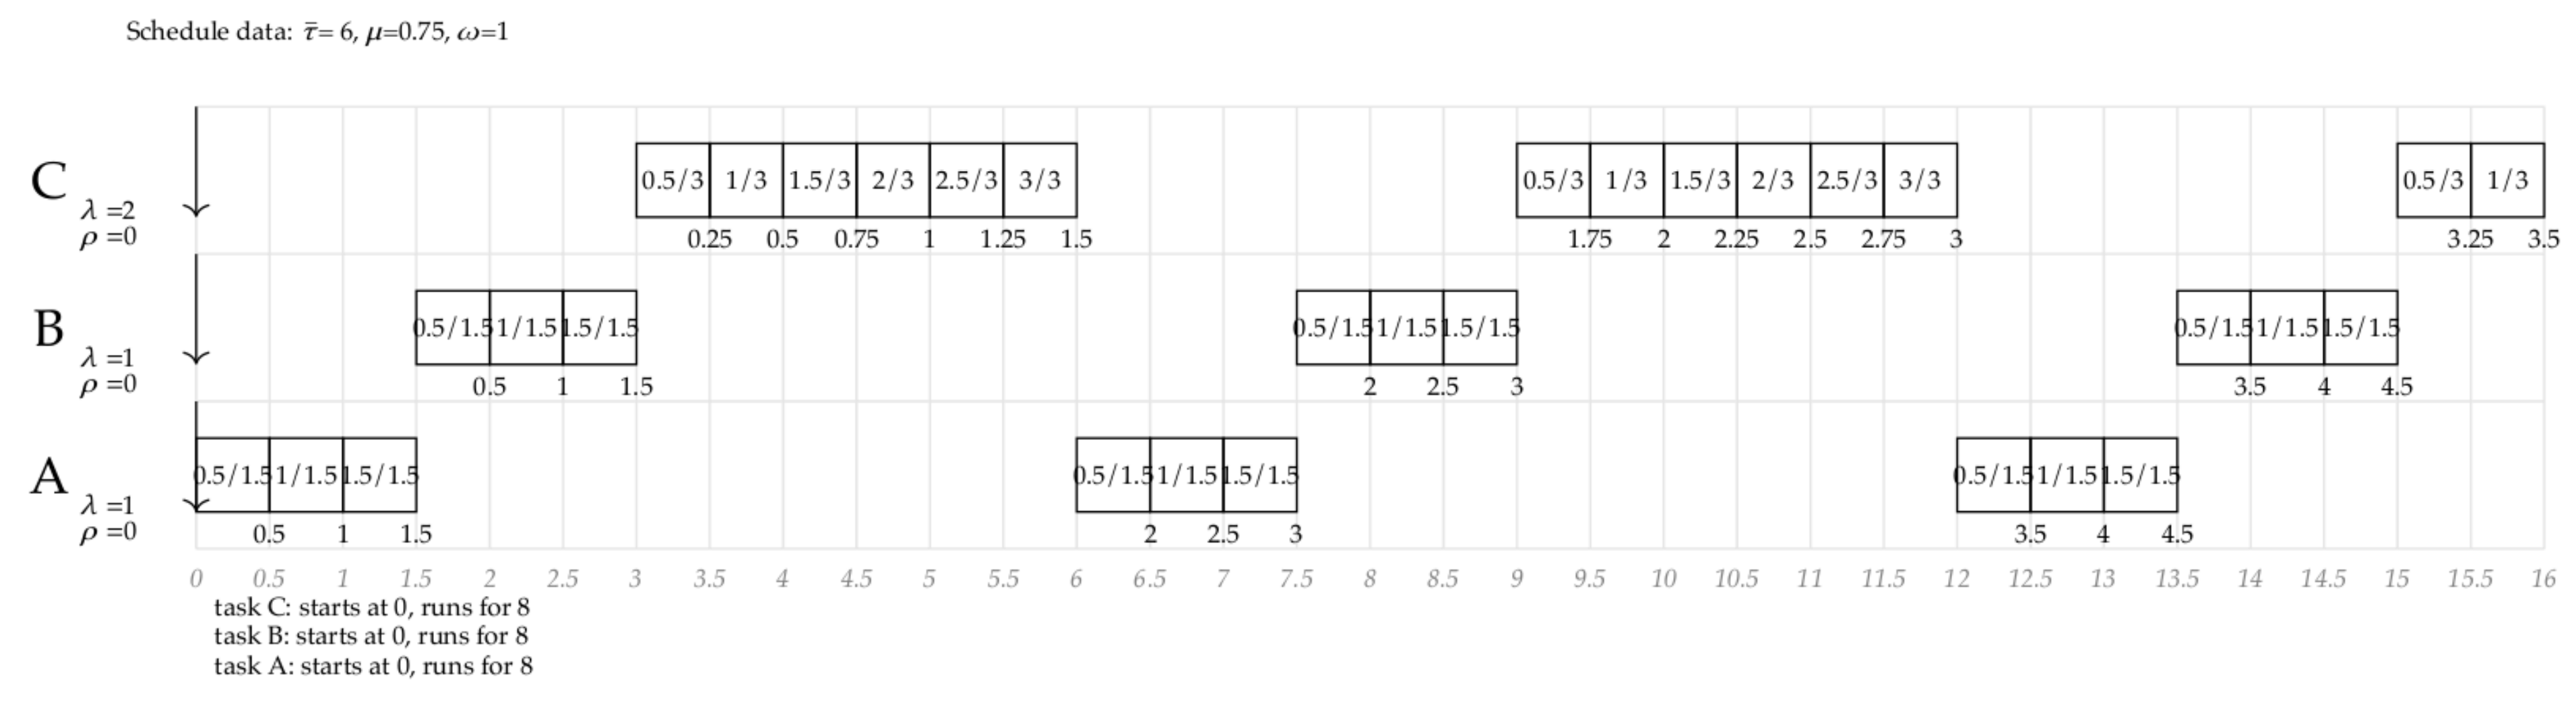
\includegraphics[width=0.75\linewidth]{images/cfs.png}
    \end{figure}
    At each timer interrupt, CFS updates the virtual runtime ($\rho_i$) and the total execution time ($\epsilon_i$) for each task based on the elapsed time ($\Delta t$) since the last update. 
    The update formula, as shown in the previous slide, governs how these values change over time.

    When a task either blocks or finishes its allocated timeslice ($\tau_i$), CFS selects the next task with the smallest $\rho$ from a red-black tree. 
    This tree efficiently manages tasks, keeping them sorted by their virtual runtime and allowing quick insertion and extraction of the minimum runtime task, both with logarithmic time complexity.
\end{example}
In summary, CFS strives to balance fairness and responsiveness by dynamically allocating CPU resources based on system load and process priority. 
However, its design does not fully accommodate tasks with specific latency requirements, leaving room for further refinement.

\subsection{Control Groups}
The CFS alone is insufficient to fully optimize CPU usage, especially in multi-user or multi-threaded environments. 
To better manage CPU resource distribution, Control Groups (CGroups) are used to limit, throttle, and account for the CPU usage of tasks. 
CGroups provide a more granular and fair way of allocating CPU resources, especially when dealing with multiple users or processes.
\begin{example}
    Consider two users: User A has 2 threads, while User B has 98 threads. 
    Without CGroups, CFS would allocate only 2\% of the CPU time to User A, which is unfair since both users should ideally receive an equal share of the CPU, regardless of the number of threads. 
    With CGroups, the CPU is divided equally between users first, and then their respective shares are distributed among their threads. 
    This prevents users with more threads from receiving an unfairly large portion of the CPU time.
\end{example}
To achieve this, the system treats each user as if they were a single task in a root run queue. 
Each user is assigned their own specific run queue, where their threads take turns consuming the user's allocated timeslice. 
This grouping of tasks into user-specific run queues is managed through CGroups.
\begin{figure}[H]
    \centering
    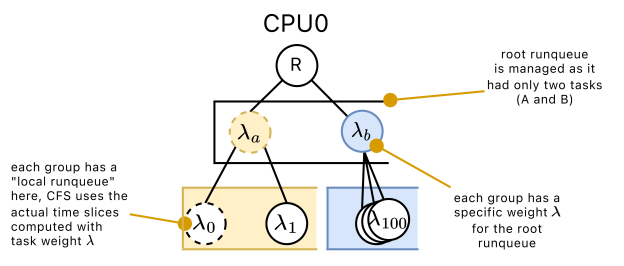
\includegraphics[width=0.75\linewidth]{images/cgroup.png}
    \caption{Control Groups implementation}
\end{figure}
The diagram illustrates how CFS integrates with CGroups to manage tasks. 
In the root run queue (e.g., CPU0), the system handles user task groups, treating them as schedulable entities similar to individual tasks. 
For example, User A and User B, although they represent task groups with multiple threads, are treated as two tasks in the root queue. 
Each user task group has its own local run queue, where tasks are scheduled independently, with CFS determining the time slices based on the weights (denoted as $\lambda$) of the tasks.

At the root level, each task group is assigned a specific weight ($\lambda$), which determines how much CPU time the group receives. 
This ensures fairness between different groups. CGroups can be nested in a hierarchical structure, allowing task groups to include other groups, all the way up to the root task group.

CGroups are particularly useful for isolating core workloads from background processes, ensuring that critical tasks are not delayed by less important jobs.

\paragraph*{CGroup creation}
The steps to create a CGroup are: 
\begin{enumerate}
    \item Create the appropriate entries in \texttt{/sys/fs/cgroup/<group name>}.
    \item Add the task's process ID (PID) to the \texttt{cgroup.procs} file.
\end{enumerate}
By managing resources through CGroups, you can fine-tune the system to ensure critical workloads receive the necessary resources without interference from background processes, leading to improved system efficiency and responsiveness.

\subsection{Load balancing}
In systems with more than one CPU, ensuring equal distribution of work, or load balancing, can become quite complex, especially when considering tasks with different priorities. 
Basic strategies like balancing based on the number of threads or the total load of each run queue are often ineffective.

For instance, balancing based solely on thread count can result in high-priority threads receiving the same CPU time as low-priority threads, which defeats the purpose of prioritization. 
Similarly, balancing based on the total load of a run queue may seem appropriate initially, but if one queue contains a high-priority thread that frequently sleeps, the CPU managing that queue may end up idle. 
This CPU would then have to steal tasks from other, more loaded CPUs, leading to inefficiency and performance degradation.

A more effective approach is to balance based on total weighted load, where both CPU usage and thread priority are considered.
By defining a process's CPU usage and computing its weighted load, a more balanced and fair distribution of CPU time is achieved. 
This method ensures that high-priority threads receive more appropriate CPU time without overwhelming the system with low-priority threads.

Let's define $\gamma_iq$ as the CPU usage of process $i$ on run queue $q$, and $\Omega^p$ as the total weighted load, calculated as:
\[\Omega^p=\sum_i\lambda_{i,q}\gamma_{i,q}\]
Here, $\lambda_{i,q}$ represents the weight (priority) of process $i$ on run queue $q$.
Balancing the system on the total weighted load, $\Omega^p$, ensures a more efficient load distribution that takes task priority into account.

To understand load balancing in Linux, it's important to consider the hierarchical layout of processor cores, caches, and memory, particularly in systems with Non-Uniform Memory Access (NUMA). 
In NUMA architectures, the memory access cost varies depending on the distance between the processor and the memory it accesses. 
If a thread is moved across different memory banks on separate dies, it incurs significant performance penalties. 
Hence, the Linux load balancer must adopt a hierarchical approach, ensuring that threads stay close to their memory and cache domains whenever possible.

To minimize these penalties, the Linux load balancer works to keep threads local to their assigned cores, caches, and memory domains, reducing latency and optimizing performance.

\paragraph*{Algorithm}
The load balancing algorithm in Linux revolves around the concept of a designated core, which is the least loaded core in the system. 
This core periodically attempts to pull tasks from the busiest cores to distribute the load more evenly.
Key steps of the algorithm:
\begin{itemize}
    \item \textit{Schedule tick}: load balancing is triggered periodically or when a core becomes idle.
    \item \textit{Walk the memory hierarchy}: the algorithm walks up the hierarchy of scheduling domains.
    \item \textit{Task stealing}: the designated core attempts to pull tasks from the busiest cores within the same scheduling domain.
\end{itemize}
At boot time, the Linux kernel gathers hardware information to understand the system's topology, such as which cores share caches and the layout of the NUMA interconnect. 
This information helps build a model of scheduling domains, which group processing units that share resources. 
Higher-level domains may span multiple cores or sockets, but moving threads across these domains incurs greater penalties.

Load balancing must also take into account the worst-case execution time of tasks, particularly for time-sensitive processes. 
In constant bandwidth scheduling, tasks are guaranteed a certain amount of CPU time. If a task exceeds its allocated time, it is throttled to prevent it from interfering with other tasks. 
However, greedy reclaiming allows tasks to use more CPU time if available, provided it doesn't violate scheduling guarantees.
By considering both CPU usage and thread priority, and ensuring tasks remain close to their memory and cache domains, Linux's load balancing mechanism maximizes performance while maintaining fairness across CPUs.